\item \points{15} {\bf Linear Classification (logistic regression)}

In this problem, we cover the linear classification task using logistic regression. The goal is to find a linear decision boundary that
separates the data into two classes. We will consider two datasets, along with starter codes provided in the following
files:
\begin{center}
\begin{itemize} %[label=\roman*.]
	\item \url{src/linearclass/ds1_{train,valid}.csv}
	\item \url{src/linearclass/ds2_{train,valid}.csv}
        \item \url{src/linearclass/logreg.py}
\end{itemize}
\end{center}
Each file contains $\nexp$ examples, one example $(x^{(i)}, y^{(i)})$ per row.
In particular, the $i$-th row contains columns $x^{(i)}_1\in\Re$,
$x^{(i)}_2\in\Re$, and $y^{(i)}\in\{0, 1\}$.

Typically, a trained model is evaluated by its performance on the validation dataset. The validation dataset is a set of examples drawn from the same (or a similar) distribution as the training data. Intuitively, this is because we need the trained model to correctly predict the label for not only the training data, but also new samples from the same distribution.

\begin{enumerate}
	\item \subquestionpoints{5}

%\textbf{TBD RETIRE THIS QUESTION? Q4c is a more generic version of this}

In lecture we saw the average empirical loss for logistic regression:
\begin{equation*}
	J(\theta)
	= -\frac{1}{\nexp} \sum_{i=1}^\nexp \left(y^{(i)}\log(h_{\theta}(x^{(i)}))
		+  (1 - y^{(i)})\log(1 - h_{\theta}(x^{(i)}))\right),
\end{equation*}
where $y^{(i)} \in \{0, 1\}$, $h_\theta(x) = g(\theta^T x)$ and
$g(z) = 1 / (1 + e^{-z})$.

Find the Hessian $H$ of this function, and show that for any vector $z$, it
holds true that
%
\begin{equation*}
    z^T H z \ge 0.
\end{equation*}
%
{\bf Hint:} You may want to start by showing that
$\sum_i\sum_j z_i x_i x_j z_j = (x^Tz)^2 \geq 0$. Recall also that
$g'(z) = g(z)(1-g(z))$.

{\bf Remark:} This is one of the standard ways of showing that the matrix $H$
is positive semi-definite, written ``$H \succeq 0$.''  This implies that $J$ is
convex, and has no local minima other than the global one. If you have some
other way of showing $H \succeq 0$, you're also welcome to use your method
instead of the one above.


        \ifnum\solutions=1 {
            \begin{answer}
\end{answer}

        } \fi

	\item \subquestionpoints{10} \textbf{Coding problem.}
In \texttt{src/linearclass/logreg.py}, write the code to train a
logistic regression classifier using Newton's Method.
Starting with $\theta = \vec{0}$, run Newton's Method until the updates to
$\theta$ are small: Specifically, train until the first iteration $k$ such
that $\|\theta_{k} - \theta_{k-1}\|_1 < \epsilon$, where
$\epsilon = 1\times 10^{-5}$. Make sure to write the model's predicted probabilities on
the validation set to the file specified in the code.

Include a plot of the \textbf{validation data} with $x_1$ on the horizontal axis and $x_2$ on the vertical axis.
To visualize the two classes, use a different symbol for examples $x^{(i)}$
with $y^{(i)} = 0$ than for those with $y^{(i)} = 1$. On the same figure, plot the decision boundary
found by logistic regression (i.e., line corresponding to $p(y|x) = 0.5$). \textbf{There is a plotting function provided in util.py.}

\textbf{Note:} If you want to print the loss during training, you may encounter some numerical instability issues. Recall that the loss function on an example $(x,y)$ is defined as
$$y\log(h_{\theta}(x)) +  (1 - y)\log(1 - h_{\theta}(x)),$$
where $h_\theta(x)=(1+\exp(-x^\top \theta))^{-1}.$ Technically speaking, $h_{\theta}(x)\in(0,1)$ for any $\theta,x\in\R^{d}.$ However, in Python a real number only has finite precision. So it is possible that in your implementation, $h_{\theta}(x)=0$ or $h_{\theta}(x)=1$, which makes the loss function ill-defined. A typical solution to the numerical instability issue is to add a small perturbation. In this case, you can compute the loss function using 
$$y\log(h_{\theta}(x) + \epsilon) +  (1 - y)\log(1 - h_{\theta}(x) + \epsilon),$$
instead, where $\epsilon$ is a very small perturbation (for example, $\epsilon=10^{-5}$).

        \ifnum\solutions=1 {
            \begin{answer}

Figure \ref{fig:logreg1} shows results for the first dataset, and Figure \ref{fig:logreg2}, for the second.
\begin{figure}
    \centering
    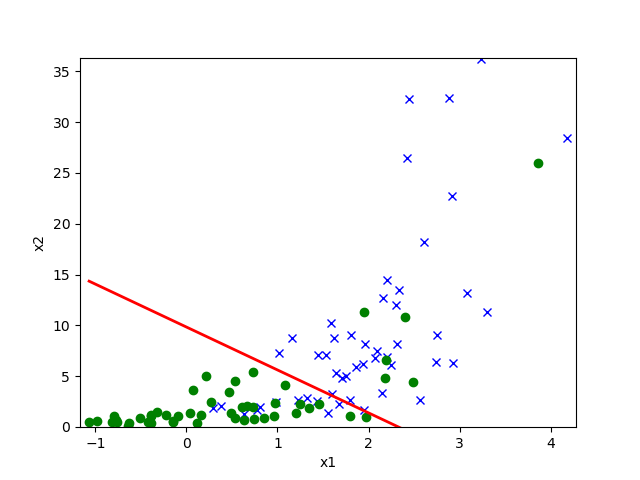
\includegraphics[width=0.75\linewidth]{ps1/tex/img/logreg_pred_1.png}
    \caption{LogReg Prediction 1}
    \label{fig:logreg1}
\end{figure}
\begin{figure}
    \centering
    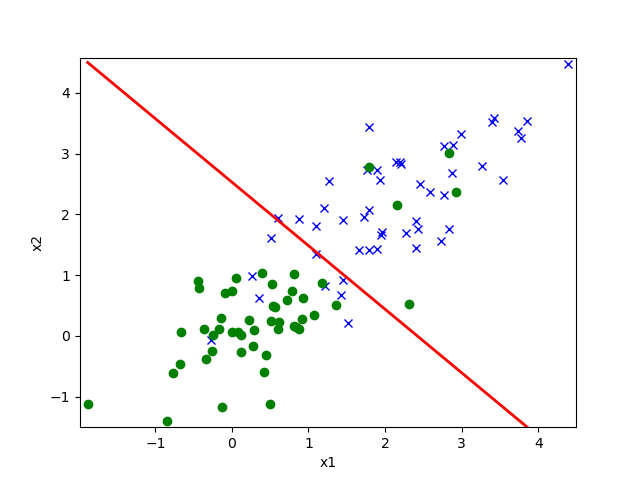
\includegraphics[width=0.75\linewidth]{ps1/tex/img/logreg_pred_2.png}
    \caption{LogReg Prediction 2}
    \label{fig:logreg2}
\end{figure}
\end{answer}

        } \fi

\end{enumerate}
